% DSD Lab3 report

\documentclass[10pt]{article}
\usepackage{mathtools, amsmath, amsfonts, amssymb}
\usepackage{hyperref, graphicx, wrapfig, geometry}
\usepackage[makeroom]{cancel}

\usepackage[section]{placeins}
\newgeometry{margin=2cm}

\title{ECSE 323 --- Group 47 Lab 4 Report Permutation}
\author{Junyoung Shin id. 260499663\\ Timothee Flichy id. 260557686}
\date{\today}

\begin{document}
\maketitle
\section{Permutation}
The permutation is used encript and revert to the original message. To do so, we were given a table which depics the character encription list given in the figure \ref{fig:permuation}. There are 4 configuration we are given to be made. To make the permutation circuit, we need 2 input and 2 outputs. The inputs will receive a 2 bit rotor\_type giving which type of encription that must be done and the second input inputs a 5 bit input\_code that must be encripted. The outputs are a 5 bit output\_code which outputs the encripted version of the input bits determined by the rotery position and the second input is the inv\_output\_code giving out the inverted or decripted 5 bit code. This is given by the figure \ref{fig:permuation_sym}.
\begin{figure}[!htb]
    \centering
    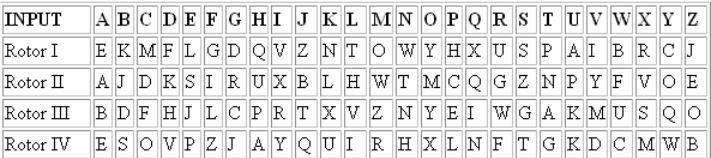
\includegraphics[width=0.5\textwidth]{./permutation.png}
    \caption{Permutation graph.}
    \label{fig:permuation}
\end{figure}
\begin{figure}[!htb]
    \centering
    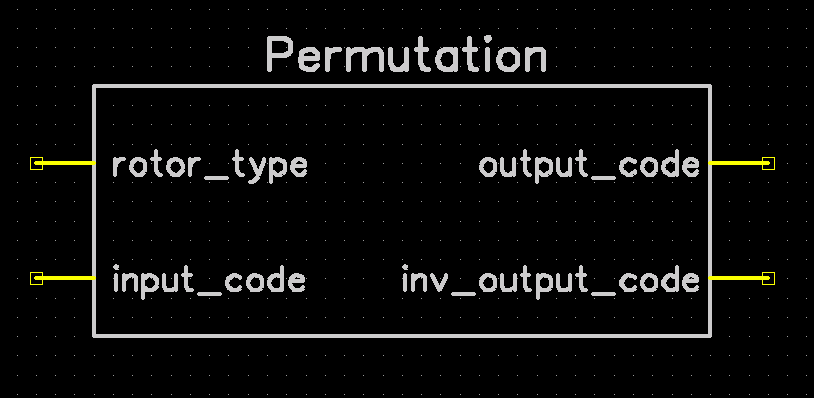
\includegraphics[width=0.5\textwidth]{./permutation_circuit.png}
    \caption{Permutation symbol.}
    \label{fig:permuation_sym}
\end{figure}
We tested out vhdl code on the ModelSim and got what we were expected to get from the permutation graph as you can see from the figures \ref{fig:perm_1}, \ref{fig:perm_2}, \ref{fig:perm_3}, \ref{fig:perm_4}, and \ref{fig:perm_5}.
\begin{figure}[!htb]
    \centering
    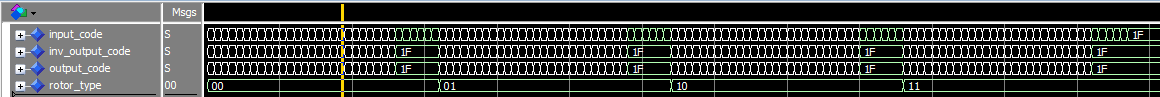
\includegraphics[width=0.5\textwidth]{./perm_1.png}
    \caption{Tested circuit on ModelSim}
    \label{fig:perm_1}
\end{figure}
\begin{figure}[!htb]
    \centering
    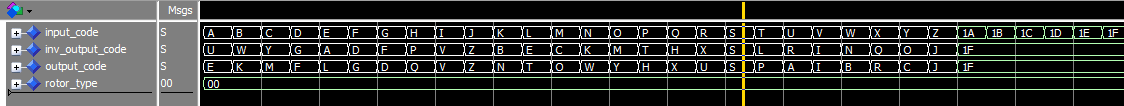
\includegraphics[width=0.5\textwidth]{./perm_2.png}
    \caption{With rotor I.}
    \label{fig:perm_2}
\end{figure}
\begin{figure}[!htb]
    \centering
    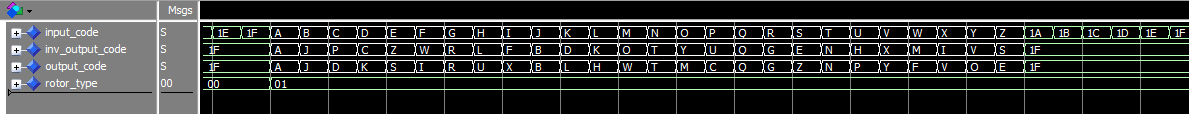
\includegraphics[width=0.5\textwidth]{./perm_3.png}
    \caption{With rotor II.}
    \label{fig:perm_3}
\end{figure}
\begin{figure}[!htb]
    \centering
    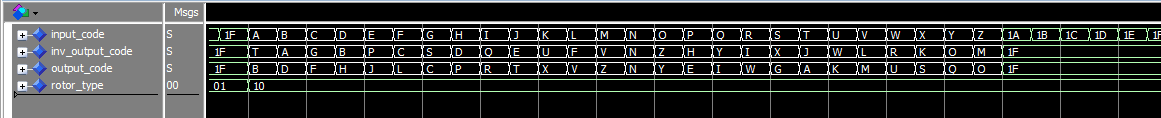
\includegraphics[width=0.5\textwidth]{./perm_4.png}
    \caption{With rotor III.}
    \label{fig:perm_4}
\end{figure}
\begin{figure}[!htb]
    \centering
    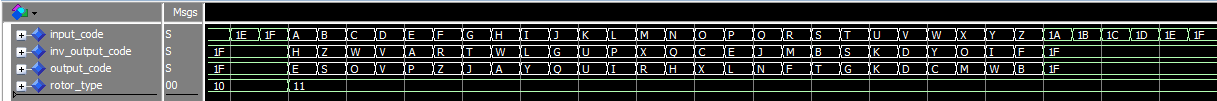
\includegraphics[width=0.5\textwidth]{./perm_5.png}
    \caption{With rotor V.}
    \label{fig:perm_5}
\end{figure}

\section{fsm}

\section{fsm_testbed}



\end{document}